% 原书 p.282–p.287（PDF p.290–p.295）
\chapter{另一种语言——层（A Different Language—Sheaf）}

% >>> p290
在前几章中我们已经看到，辛几何中的许多理论都建立在伪全纯曲线的研究之上，它们通过
建立各种新颖的辛刚性来显示自身的力量。本章中，我们将引入一个基于层论的新框架；与
伪全纯曲线不同，它同时也有利于研究辛几何的各个方面。特别地，目前（层）复形与核心
辛对象之间已有良好建立的对应关系，这些对象包括拉格朗日子流形、哈密顿微分同胚以及
刘维尔区域（例如在欧氏空间中）。值得注意的是，层之间的代数运算能够还原笛卡尔积、
拉格朗日对应、由哈密顿流实现的位移等几何运算。这把一个几何问题转化为代数问题，这一
过程常被称为\textbf{层量子化}（sheaf quantization）。追溯其源，以这种方式使用层，其
灵感来自生成函数方法（见 10.1 节），并由 M.~Kashiwara 与 P.~Schapira 基于微局部分析
的思想严格发展起来。特别地，奇性支撑（singular support，见 10.6 节）这一概念是把代数
与几何联系起来的核心概念。

\section{生成函数（Generating Function）}

% >>> p291
生成函数方法是辛几何中最古老的技术之一，起源于 20 世纪 70 年代 [126]，早于 Floer
理论。其核心思想是把（子）流形转化为函数，使相应函数的临界点获得几何／动力学意义，
从而推出（子）流形某些所需的刚性。

给定光滑流形 $Q$ 上的光滑函数 $f\colon Q\to\R$，回忆例 1.6.3 中的图像
\begin{equation}\tag{10.1}
  \operatorname{graph}(\dd f)=\{(x,\dd f(x))\mid x\in Q\}\subset T^*Q
\end{equation}
是 $(T^*Q,\omega_{\mathrm{can}})$ 中的拉格朗日子流形。换言之，拉格朗日子流形
$\operatorname{graph}(\dd f)$ 承认一个「\textbf{生成函数}」$f$。当然，人们可以问
相反的问题：给定拉格朗日子流形 $L\subset(T^*Q,\omega_{\mathrm{can}})$，是否可以把
$L$ 写成 $Q$ 上某个函数的图像？答案显然是否定的！下面是一个简单的例子。

\begin{keytakeaways}
\begin{itemize}
  \item 几何图像：把拉格朗日子流形「参数化」为某个函数的图像——若不行，就添加额外
        的欧氏空间 $\R^N$，用「纤维上的临界条件」把多余的变量消去。
  \item 数学工具：生成函数 $F\colon Q\times\R^N\to\R$，$L$ 由
        $(x,\partial_xF(x,e))$（其中 $\partial_eF(x,e)=0$）给出；以及
        Hamilton--Jacobi 意义下的作用量公式 $F=\int_0^1(\lambda_{\mathrm{can}}(X_{H_t})-H_t)\circ\varphi_H^t\,\dd t$。
  \item 关键定理：定理 10.1.1 断言与零截面哈密顿同痕的拉格朗日子流形必有生成函数，
        且生成函数在无穷远处为二次型；由此得到推论 10.1.1（拉格朗日 Arnold 猜想的一个
        特殊情形）。
  \item 本节结论：生成函数在复合下变得复杂（命题 10.1.1），而任意哈密顿同痕可分解为
        $C^1$-小的哈密顿同痕之积（式 (10.5)），这为下一节引入层语言埋下伏笔。
\end{itemize}
\end{keytakeaways}

\begin{wexam}{10.1.1}
  考虑图 10.1 所示的拉格朗日 $L\subset(T^*\R,\omega_{\mathrm{can}})$。显然，$L$
  甚至不是光滑的，它有一个奇点 $(0,0)$。此外，作为图像，它必须满足 $T^*\R$ 中的
  「竖直线检验」：换言之，任意竖直线 $q=q_\ast$ 至多与 $L$ 相交一次。因此，作为
  拉格朗日子集（即 $\omega_{\mathrm{can}}$ 在其上为零），$L$ 不可能具有 (10.1)
  形式的图像表示。
  \hfill$//$
\end{wexam}

\begin{figure}[htbp]
  \centering
  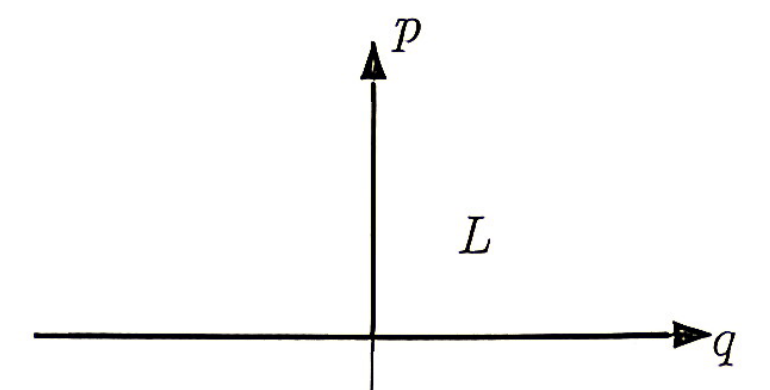
\includegraphics[width=0.42\linewidth]{figures/fig_p291_1.png}
  \caption*{图 10.1\quad $\R^2$ 中的一个拉格朗日（原书 p.283, Figure 10.1；PDF p.291）}
\end{figure}

这里有一个革命性的做法：它修改例 10.1.1，使得我们能够把例 10.1.1 中的 $L$ 写成
图像（但需要一些额外的输入）。关键的一步是给底流形添加额外的（欧氏）空间，即把
$Q$ 换成 $Q\times\R^N$（$N$ 充分大）。作为例子，对例 10.1.1 考虑
$\R\times\R^1$。记 $e$ 为额外空间 $\R^1$ 的坐标，并考虑由下式定义的
$F\colon\R\times\R^1\to\R$：
\[
  F(x,e)=xe^2.
\]
则例 10.1.1 中的 $L$ 可以用 $F$ 表示如下：
\begin{equation}\tag{10.2}
  L=\left\{\left.\left(x,\frac{\partial F}{\partial x}(x,e)\right)
  \;\right|\;(x,e)\ \text{满足}\
  \frac{\partial F}{\partial e}(x,e)=0\right\}.
\end{equation}
确实，$\frac{\partial F}{\partial e}(x,e)=0$ 等价于 $x=0$ 或 $e=0$。于是由
$\frac{\partial F}{\partial x}=e^2$，在 $(x,e)=(0,e)$ 或 $(x,e)=(x,0)$ 处取值，
(10.2) 的右端等于 $T^*\R$ 的下述子集：
\[
  \{(0,p)\in T^*\R\mid p=e^2\ge0\}
  \cup\{(x,0)\in T^*\R\mid x\in\R\},
\]
它与图 10.1 中的 $L$ 重合。这样，$L$ 就可以看作 $\dd F$ 的图像，只不过它被额外
欧氏空间 $\R^1$ 中的临界纤维切了出来。

\begin{wrem}{10.1.1}
  经过足够多类似例 10.1.1 的修改练习之后，人们会获得一种大致的感受：把 $Q$ 升级为
  $Q\times\R^N$ 时所需的额外空间 $\R^N$（就其维数 $N$ 而言）有多复杂，取决于 $L$
  有多「非图像化」。
\end{wrem}

% [Tutor Note: 含糊点拨——例 10.1.1 的处理是「生成函数族」（generating family）思想
% 的雏形：先在 $Q\times\R^N$ 上取一个普通函数 $F$，再只保留 $\partial_eF=0$ 的临界
% 纤维上的信息，投影到 $T^*Q$。$N$ 的大小反映 $L$ 的「复杂度」：若 $L$ 是某个函数的
% 图像则 $N=0$；一般 $L$ 需要 $N$ 来「解耦」其多值性。特别地，$F$ 在
% $\operatorname{Crit}(\partial_eF)$ 上的图像才落进 $T^*Q$，这就是 (10.2) 中先取
% $\partial_xF$、再要求 $\partial_eF=0$ 的原因。]

基于添加额外空间的想法，我们可以给出与余切丛中拉格朗日子流形相伴的生成函数的下述定义。

% >>> p292
\begin{wdefn}{10.1.1}
  设 $L\subset(T^*Q,\omega_{\mathrm{can}})$ 是拉格朗日子流形。若存在整数 $N\in\N$
  与可微函数 $F\colon Q\times\R^N\to\R$，使得
  \begin{equation}\tag{10.3}
    L=\left\{\left.\left(x,\frac{\partial F}{\partial x}(x,e)\right)
    \;\right|\;(x,e)\ \text{满足}\
    \frac{\partial F}{\partial e}(x,e)=0\right\},
  \end{equation}
  则称 $L$ \textbf{承认一个生成函数}。当 $N=0$ 时，(10.3) 中的条件为空，
  $L=\operatorname{graph}(\dd F)$。
\end{wdefn}

% [Tutor Note: 易错预警——定义 10.1.1 中 $F$ 的变量分为两组：$x\in Q$ 是底流形坐标，
% $e\in\R^N$ 是额外（纤维）坐标。$L$ 由「$e$ 方向的临界点处对 $x$ 求导」得到，
% 而不是对全部变量求导：$\dd F$ 在 $\operatorname{Crit}(\partial_eF)$ 上的图像投影
% 到 $T^*Q$ 才是 $L$。若误把条件写成 $\dd F=0$，得到的是 $L$ 与零截面的交点而非
% $L$ 本身。另注意 $N$ 并非唯一（见注 10.1.2），故生成函数不唯一，这正是后面要用
% 「层」这种对 $N$ 不敏感的对象的动机。]

\begin{wrem}{10.1.2}
  注意：若拉格朗日 $L\subset(T^*Q,\omega_{\mathrm{can}})$ 承认生成函数
  $F\colon Q\times\R^N\to\R$，则通过平凡地增大额外空间的维数至 $\R^{N'}$
  （$N'\ge N$），并定义 $F'\colon Q\times\R^{N'}\to\R$ 为
  \[
    F'(q,e_1,\cdots,e_{N'})=F(q,e_1,\cdots,e_N),
  \]
  便得到 $L$ 的另一个生成函数 $F'$。因此，$L$ 的生成函数（若存在）有无穷多个。
\end{wrem}

下面这个例子表明，生成函数也自然地出现在哈密顿动力学中。

\begin{wexam}{10.1.2}[cf.\ 考试 III 中的问题 A]
  设 $L\subset(T^*Q,\omega_{\mathrm{can}}=\dd\lambda_{\mathrm{can}})$ 是
  $C^1$-小的哈密顿微分同胚 $\varphi_H^1$（即相应的哈密顿函数在 $H_t$ 与
  $\dd H_t$ 上都很小）作用在零截面 $0_Q$ 上的像。则 $L$ 可以看作某个恰当 1-形式
  $\sigma=\dd F$ 的图像，其中 $F\colon Q\to\R$ 可以显式地写成
  \[
    F=\left(\int_0^1\left(\lambda_{\mathrm{can}}(X_{H_t})-H_t\right)
    \circ\varphi_H^t\,\dd t\right).
  \]
  换言之，$L=\operatorname{graph}(\dd F)$，且由定义 10.1.1，$F$ 是 $L$ 的一个生成
  函数。重要的是，这意味着 $L$ 与 $0_Q$ 的交点与 $F$ 的临界点（即满足
  $\dd F(q)=0$ 的 $q\in Q$）一一对应。特别地，若 $Q$ 紧，则由该对应关系有
  \begin{equation}\tag{10.4}
    L\cap 0_Q=\varphi_H^1(0_Q)\cap 0_Q\ne\varnothing.
  \end{equation}
  当 $\varphi_H^1$ 不是 $C^1$-小时，上述论证失效（此时 $L$ 可能不是图像），需要
  额外欧氏空间才能完成上面例 10.1.1 中讨论的修改。
  \hfill$//$
\end{wexam}

% [Tutor Note: 易错预警——例 10.1.2 中的 $F$ 正是作用量泛函在「图」上的取值：
% 对路径 $\varphi_H^t(q)$ 积分 $\lambda_{\mathrm{can}}(X_{H_t})-H_t$，即作用量
% $\int_0^1(\lambda_{\mathrm{can}}(\dot x)-H_t)\,\dd t$（因为
% $\dot x=X_{H_t}\circ\varphi_H^t$）。因此 $L=\operatorname{graph}(\dd F)$ 就是
% Hamilton--Jacobi 方程 $\dd F=\lambda_{\mathrm{can}}(X_H)-H$ 的全局解；
% (10.4) 则是「$F$ 在紧流形上必有临界点」的推论。核对时注意 $\lambda_{\mathrm{can}}$
% 的符号约定（$\omega_{\mathrm{can}}=\dd\lambda_{\mathrm{can}}$，且
% $\lambda_{\mathrm{can}}=\sum p_i\,\dd q_i$），以及 $H_t$ 的系数为 $-1$。]

\begin{wrem}{10.1.3}
  由于定义 10.1.1 中的额外欧氏空间，显式地构造／写出一个生成函数几乎是不可能的。
  许多结果都是在假设生成函数存在的前提下证明的。
\end{wrem}

下述里程碑式的成果是例 10.1.2 的推广。它的力量在于去掉了例 10.1.2 中的
$C^1$-小条件（但增加了底流形 $Q$ 的复杂性：$Q$ 被换成 $Q\times\R^N$，其中
$N\in\N$ 充分大）。

% >>> p293
下述结果的证明冗长且超出本书范围。我们只强调：额外空间 $\R^N$ 的维数 $N$ 来自一个
归纳论证（因此 $N$ 的确切取值并不完全清楚）。

\begin{wthm}{10.1.1（[143, 206--207]）}
  若 $L\subset(T^*Q,\omega_{\mathrm{can}})$ 与零截面 $0_Q$ 哈密顿同痕（即
  $L=\varphi_H^1(0_Q)$，其中 $H\colon[0,1]\times Q\to\R$ 是某个哈密顿函数），则
  存在 $N\in\N$，使 $L$ 承认生成函数 $F\colon Q\times\R^N\to\R$。此外，在
  $\R^N$ 的某个紧子集 $K$ 之外，$F$ 满足
  \[
    F(x,e)=\sum_{i=1}^{N}\pm e_i^2,
  \]
  它对任意 $x\in Q$ 与 $e\in\R^N\setminus K$ 是一个二次型。
\end{wthm}

% [Tutor Note: 含糊点拨——定理 10.1.1 是生成函数理论的基本存在性定理（Chaperon、
% Laudenbach--Sikorav、Viterbo 等工作；[143, 206--207] 为相应文献）。两个要点：
% (i)「$F$ 在无穷远处为二次型」这一条件保证 $\partial_eF=0$ 的临界集在纤维方向是
% 紧的（properness），从而 (10.3) 定义出的 $L$ 是良好行为的拉格朗日子流形，也是
% Floer/层理论中紧性论证的前提；(ii) $N$ 由归纳得到，故一般不可显式控制——这正是
% 注 10.1.3 说显式构造几乎不可能的原因。证明通常把 Hamiltonian 同痕分解为
% $C^1$-小块，再用「二次型 + 小扰动」的 Lagrange 乘子逐步归纳。]

沿用上面 (10.4) 的精神，下述版本的拉格朗日 Arnold 猜想是定理 10.1.1 的直接推论；
它用拉格朗日子流形刻画哈密顿微分同胚的刚性。这是所谓 \textbf{Arnold--Givental 猜想}
的一个特殊情形（见定理 10.8.1 与注 10.8.1）。

\begin{wcor}{10.1.1}
  设 $Q$ 是紧流形，$0_Q$ 表示余切丛 $(T^*Q,\omega_{\mathrm{can}})$ 的零截面。则对
  任意哈密顿微分同胚 $\varphi_H^1$，有
  \[
    \varphi_H^1(0_Q)\cap 0_Q\ne\varnothing.
  \]
\end{wcor}

\begin{wproof}
  令 $L:=\varphi_H^1(0_Q)$，按定义它与零截面 $0_Q$ 哈密顿同痕。于是由定理 10.1.1，
  $L$ 承认生成函数 $F\colon Q\times\R^N\to\R$。观察到：由 $L$ 的表达式 (10.3)，
  存在一一对应
  \[
    \varphi_H^1(0_Q)\cap 0_Q\longleftrightarrow\Crit(F),
  \]
  其中 $\Crit(F)$ 由 $F$ 在 $Q\times\R^N$ 中的临界点组成。确实，对任意
  $(x,p)\in\varphi_H^1(0_Q)\cap 0_Q$，有
  \[
    p=\frac{\partial F}{\partial x}(x,e)=0,
  \]
  这蕴含 $(x,e)$ 是 $F$ 的临界点；反之亦然。

  此外，由定理 10.1.1 的第二个结论，存在紧子集 $K$，使得对任意 $x\in Q$ 与
  $e\in\R^N\setminus K$ 有 $F(x,e)=\sum_{i=1}^N\pm e_i^2$。于是
  \[
    \frac{\partial F}{\partial e_i}(x,e)=0
    \quad\Longrightarrow\quad e_i=0
    \ \text{对任意}\ i=1,\cdots,N.
  \]
  我们可以把紧集 $K$ 放大，使得 $0\in K$。由上述讨论，在 $Q\times(\R^N\setminus K)$
  中临界点必须形如 $(x,0)$，这与 $0\notin\R^N\setminus K$ 矛盾。这意味着 $F$ 的
  任何临界点都必须来自紧集 $Q\times K$，而后者由紧性总是存在的。于是由上述一一对应，
  我们断定 $\varphi_H^1(0_Q)\cap 0_Q\ne\varnothing$。
\end{wproof}

% >>> p294
注意：定义 10.1.1 只对余切丛中的拉格朗日子流形定义了生成函数。一个自然的问题是：
能否对其他对象定义生成函数？例如，辛流形 $(M,\omega)$ 上的哈密顿微分同胚
$\varphi=\varphi_H^1$ 如何？朴素的做法是考虑图像
\[
  \operatorname{graph}(\varphi)=\{(x,\varphi(x))\in M\times M\mid x\in M\},
\]
其中 $(M\times M,\omega_{\mathrm{twisted}})$ 是配有扭辛结构的乘积辛流形（见练习
1.2.2 与例 1.6.2）。然后应用 Weinstein 邻域定理（定理 4.3.3），把对角
$\Delta\subset(M\times M,\omega_{\mathrm{twisted}})$ 的邻域转移到零截面
$0_M\subset(T^*M,\omega_{\mathrm{can}})$ 的邻域。于是，对含于 $\Delta$ 的邻域中、
作为 $(T^*M,\omega_{\mathrm{can}})$ 的拉格朗日子流形的
$\operatorname{graph}(\varphi)$ 的像，定义 10.1.1 适用。

不幸的是，这只对 $C^1$-小的哈密顿微分同胚 $\varphi$ 有效，此时
$\operatorname{graph}(\varphi)$ 落在对角 $\Delta$ 的一个（就定理 4.3.3 而言）可用
的邻域中。一般而言，无法预测 $\operatorname{graph}(\varphi)$ 能伸出去多远。下面
这个例子说明了一种情形：从 $(M\times M,\omega_{\mathrm{twisted}})$ 到
$(T^*M,\omega_{\mathrm{can}})$ 的变换可以整体地实现。

\begin{wexam}{10.1.3}[哈密顿微分同胚的生成函数，[197] 第 7 节]
  设 $\varphi$ 是 $(\R^{2n},\omega_{\mathrm{std}})$ 上的哈密顿微分同胚。回忆
  \[
    \operatorname{graph}(\varphi)=\{(x,\varphi(x))\mid x\in\R^{2n}\}
    \subset(\R^{2n}\times\R^{2n},-\omega_{\mathrm{std}}\oplus\omega_{\mathrm{std}})
  \]
  是 $(\R^{2n}\times\R^{2n},-\omega_{\mathrm{std}}\oplus\omega_{\mathrm{std}})$ 中的
  拉格朗日子流形。考虑下述映射
  \begin{align*}
    \tau\colon(\R^{2n}\times\R^{2n},-\omega_{\mathrm{std}}\oplus\omega_{\mathrm{std}})
    &\longrightarrow(T^*\R^{2n},\omega_{\mathrm{can}})\\
    (x,y,X,Y)&\longmapsto
    \left(\frac{x+X}{2},\frac{y+Y}{2},Y-y,x-X\right),
  \end{align*}
  其中 $(Y-y,x-X)$ 是 $T^*_{(x+X)/2,(y+Y)/2}\R^{2n}$ 处的余向量。于是可以验证
  $\tau$ 实际上是辛同胚，因为
  \begin{align*}
    \tau^*\omega_{\mathrm{can}}
    &=\left(\frac{\dd x+\dd X}{2}\right)\wedge(\dd Y-\dd y)
    +\left(\frac{\dd y+\dd Y}{2}\right)\wedge(\dd x-\dd X)\\
    &=-\dd x\wedge\dd y+\dd X\wedge\dd Y=\omega_{\mathrm{std}}.
  \end{align*}
  因此，$\tau(\operatorname{graph}(\varphi))
  \subset(T^*\R^{2n},\omega_{\mathrm{can}})$ 是拉格朗日子流形。于是，可以经由所得
  拉格朗日子流形 $\tau(\operatorname{graph}(\varphi))$ 的生成函数，来定义
  $(\R^{2n},\omega_{\mathrm{std}})$ 上哈密顿微分同胚 $\varphi$ 的生成函数。
  \hfill$//$
\end{wexam}

% [Tutor Note: 易错预警——$\tau$ 的公式中前两个分量
% $(\frac{x+X}{2},\frac{y+Y}{2})$ 是 $T^*\R^{2n}$ 的底坐标 $q$，后两个分量
% $(Y-y,x-X)$ 是纤维坐标 $p$。核对 $\tau^*\omega_{\mathrm{can}}=\omega_{\mathrm{std}}$
% 时，要把 $\omega_{\mathrm{can}}=\sum\dd q_i\wedge\dd p_i$ 按
% $q=(q_1,q_2)$、$p=(p_1,p_2)$ 展开，其中 $q_1=(x+X)/2$、$q_2=(y+Y)/2$、
% $p_1=Y-y$、$p_2=x-X$；四次叉积中 $\dd x\wedge\dd Y$ 等交叉项相消，只剩
% $-\dd x\wedge\dd y+\dd X\wedge\dd Y$。注意符号：$-\omega_{\mathrm{std}}\oplus
% \omega_{\mathrm{std}}$ 的负号进入第一个因子，故结果为 $-\dd x\wedge\dd y$。
% 另外 $\tau$ 实际上是「差—和」型的线性辛同胚（属 $Sp$ 的某个子群），可用分块矩阵
% 验证。]

为结束本节，我们提及另一个重要的观察（第一作者 2016 年从 L.~Polterovich 处得知），
它启发了从下一节开始引入的层：任意哈密顿同痕 $\{\varphi_t\}_{t\in[0,1]}$ 都可以分解为
$C^1$-小哈密顿同痕的乘积。显式地说，
\begin{equation}\tag{10.5}
  \{\varphi_t\}_{t\in[0,1]}
  =\prod_{i=1}^{N}\{\psi_t^{(i)}\}_{t\in[0,1]},
  \qquad\text{其中}\quad
  \psi_t^{(i)}=\varphi_{\frac{(i-1)t}{N}}\circ\varphi_{\frac{it}{N}}^{-1},
\end{equation}
% >>> p295
其中 $N$ 可以取得充分大（使每个 $\psi_t^{(i)}$ 都是 $C^1$-小的）。因此，结合例
10.1.2，若要从 $C^1$-小的哈密顿微分同胚出发计算一般哈密顿微分同胚的生成函数，就
需要理解生成函数在 (10.5) 那样的微分同胚复合之下如何变化。一般说来这相当复杂，下面
的命题即使在相当初等的框架下也展示了这种复杂性。

% [Tutor Note: 原文疑误——按 (10.5) 的写法
% $\psi_t^{(i)}=\varphi_{(i-1)t/N}\circ\varphi_{it/N}^{-1}$，若按通常的复合次序
% 取乘积 $\psi^{(1)}\circ\cdots\circ\psi^{(N)}$，则对 $N=2$ 得
% $\psi^{(1)}\circ\psi^{(2)}=\varphi_t^{-1}$，一般地得到 $\varphi_t^{-1}$ 而非
% $\varphi_t$。欲使乘积真正伸缩相消为 $\varphi_t$，应取
% $\psi_t^{(i)}=\varphi_{it/N}\circ\varphi_{(i-1)t/N}^{-1}$（或等价地把复合次序
% 反过来）。此处译文保留原文写法；已记入 review_ch10a.md，建议核对原书。]

\begin{wprop}{10.1.1（[97] 中的命题 2.2）}
  设 $F_1\colon\R^{2n}\times\R^{N_1}\to\R$ 是哈密顿微分同胚 $\varphi_1$ 的生成
  函数，$F_2\colon\R^{2n}\times\R^{N_1}\to\R$ 是哈密顿微分同胚 $\varphi_2$ 的
  生成函数。则复合 $\varphi_2\circ\varphi_1$ 有生成函数
  \[
    F_1\#F_2\colon\R^{2n}\times(\R^{2n}\times\R^{2n}\times\R^{N_1}\times\R^{N_2})
    \to\R,
  \]
  定义为
  \[
    (F_1\#F_2)\bigl(q,(q_1,q_2,e_1,e_2)\bigr)
    =F_1(q_1,e_1)+F_2(q_2,e_2)
    -2\bigl\langle q_2-q,\sqrt{-1}(q_1-q)\bigr\rangle,
  \]
  其中
  $(q,(q_1,q_2,e_1,e_2))\in\R^{2n}\times(\R^{2n}\times\R^{2n}\times\R^{N_1}
  \times\R^{N_2})$，而 $\sqrt{-1}$ 是 $\C^n\simeq\R^{2n}$ 上的复结构，满足
  对 $(A,B)\in\R^{2n}$ 有 $\sqrt{-1}(A,B)=(-B,A)$。
\end{wprop}

% [Tutor Note: 原文疑误——命题 10.1.1 中第二个生成函数的类型印作
% $F_2\colon\R^{2n}\times\R^{N_1}\to\R$，但 $F_1\#F_2$ 的定义里 $e_2$ 取值于
% $\R^{N_2}$，故 $F_2$ 的定义域应为 $\R^{2n}\times\R^{N_2}$。已记入
% review_ch10a.md，建议核对原书。]
% [Tutor Note: 含糊点拨——$\#$-积（fiber sum）的公式可以这样理解：
% $F_1(q_1,e_1)+F_2(q_2,e_2)$ 是两张「图」的直和，而
% $-2\langle q_2-q,\sqrt{-1}(q_1-q)\rangle$ 是迫使中间变量 $q_1,q_2$ 逼近同一
% 点的耦合项（其临界条件同时给出 $q$ 的对称化与辛结构的旋转）。核对时注意
% $\langle\cdot,\cdot\rangle$ 是 $\R^{2n}$ 上的标准内积，$\sqrt{-1}$ 作为
% $90^\circ$ 旋转起作用；符号 $-$ 与因子 $2$ 是使临界点恰好给出
% $\varphi_2\circ\varphi_1$ 的图像所需。]

在本章接下来的内容中，通过层的语言，这样一个复杂的复合公式会转化为层之间的标准运算，
这使我们得以讨论哈密顿微分同胚的层版本（称为 \textbf{GKS-层量子化}，见定理 10.6.1）。
